%%%%%%%%%%%%%%%%%%%%%%%%%%%%%%%%%%%%%%%%%%%%%%%%%%%%%%%%%%%%%%%%%%%%%%
% How to use writeLaTeX: 
%
% You edit the source code here on the left, and the preview on the
% right shows you the result within a few seconds.
%
% Bookmark this page and share the URL with your co-authors. They can
% edit at the same time!
%
% You can upload figures, bibliographies, custom classes and
% styles using the files menu.
%
%%%%%%%%%%%%%%%%%%%%%%%%%%%%%%%%%%%%%%%%%%%%%%%%%%%%%%%%%%%%%%%%%%%%%%

\documentclass[12pt]{article}

\usepackage{sbc-template}

\usepackage{graphicx,url}

%\usepackage[brazil]{babel}   
\usepackage[utf8]{inputenc}  

     
\sloppy

\title{Detecção de eixos de caminhões}

\author{Matheus Peixoto Ribeiro Vieira - 22.1.4104}


\address{Departamento de Computação (DECOM) -- Universidade Federal de Ouro Preto (UFOP)
  \email{matheus.peixoto@aluno.ufop.edu.br}
}

\begin{document} 

\maketitle

\begin{abstract}
    Road transportation in Brazil features a large number of heavy vehicles in circulation, which can cause excessive wear and tear on the roads. In this context, the implementation of effective techniques to monitor the traffic of these vehicles becomes essential. Many cities impose restrictions not only based on the total gross weight but also considering the number of axles. In this regard, convolutional neural networks emerge as a promising tool for identifying the number of axles of heavy vehicles through images. This study aims to explore the use of these techniques to address the issue of vehicle monitoring and classification, contributing to the preservation of public roads.
\end{abstract}
     
\begin{resumo} 
    O transporte rodoviário no Brasil apresenta uma grande quantidade de veículos pesados em circulação, o que pode causar desgastes excessivos nas estradas. Nesse contexto, torna-se essencial a implementação de técnicas eficazes para fiscalizar o trânsito desses veículos. Muitas cidades adotam restrições não apenas com base no peso bruto total, mas também considerando a quantidade de eixos. Nesse sentido, as redes neurais convolucionais surgem como uma ferramenta promissora para identificar a quantidade de eixos de veículos pesados por meio de imagens. Este trabalho tem como objetivo explorar o uso dessas técnicas para solucionar o problema de fiscalização e classificação de veículos, contribuindo para a preservação das vias públicas.
\end{resumo}


\section{Introdução}
    Segundo o Conselho Nacional de Trânsito (CONTRAN), o transporte de cargas em veículos pesados está sujeito a limites para o Peso Bruto Total Combinado (PBTC), que corresponde à soma do peso do veículo, sua carroceria e a carga transportada. Nesse contexto, veículos de três eixos do tipo semirreboque podem atingir um PBTC máximo de 25,5 toneladas, enquanto veículos de quatro eixos têm limite de até 58,5 toneladas \cite{resolucao_contran}.
    
    Conforme discutido em \cite{damage_on_roads}, o tráfego de veículos leves e pesados em trechos rodoviários pode causar danos às estradas, sendo que os veículos de maior peso exercem um impacto significativo sobre as condições do pavimento, acelerando sua deterioração ao longo do tempo.
    
    Para mitigar esses impactos, diversas cidades brasileiras restringem a circulação de veículos pesados em áreas urbanas, visando preservar as vias públicas. Um exemplo disso ocorreu em Coronel Fabriciano, Minas Gerais, onde o Decreto Municipal nº 8.472/2023 proibiu a passagem de veículos com peso bruto total acima de 23 toneladas e aqueles com mais de três eixos em vias de quatro bairros específicos \cite{prefeitura_de_coronel_fabriciano}.
    
    Para auxiliar na fiscalização do trânsito em diferentes áreas, este trabalho explora a hipótese de que redes neurais convolucionais podem ser utilizadas para identificar a quantidade de eixos dos veículos. Essa abordagem é fundamentada no fato de que essas redes já demonstraram excelentes resultados na identificação de diferentes classes de veículos, conforme apresentado em \cite{iluminacao_adversa}, e na contagem de eixos, conforme explorado em \cite{marcomini2023truckaxledetectionconvolutional}.

\section{Trabalhos relacionados}

    Os caminhões podem variar em tamanho, tipo de carga e configuração da cabine. Para classificar essas características, \cite{Almutairi2022} utilizou imagens laterais de veículos capturadas pelo Departamento de Transporte da Flórida. O estudo, focado na classificação do tipo de caminhão com base nos critérios da Federated Highway Administration, alcançou 89\% de acurácia no conjunto de testes usando o modelo Inception V3.

    Nem sempre as condições de iluminação são propicias e, levando este fator em consideração, \cite{iluminacao_adversa} criou um dataset com condições de iluminação adversas para classificar tipos de veículos. O treinamento envolveu diferentes modelos com redes convolucionais pré-treinadas, obtendo melhores resultados com uma ResNet, atingindo um resultado de 99.68\%.

    Mesmo possuindo imagens laterais, nem sempre elas obterão uma visão completa dos veículos, que podem não caber por completo na imagem. Dessa forma, \cite{Souza2024} propôs um algoritmo para reconstruir uma imagem com diferentes quadros de um vídeo a partir da passagem de um veículo. Em seguida, utilizando o YOLO foi detectado a quantidade de eixos dos veículos que estavam passando, obtendo melhores resultados com o YOLOv5m.

    Além de se preocupar com a contagem de eixos, \cite{Miles2022} também se preocupou com a velocidade dos veículos, ao mesmo tempo que se preocupava com a não visibilidade dos eixos de todos os veículos. Dessa forma, utilizando a YOLOv4 e, ignorando veículos que não era possível identificar todos os eixos, foi obtido um mAP de 93.3\% nas imagens de teste.

    Por fim, \cite{marcomini2023truckaxledetectionconvolutional} decidiu investigar diferentes arquiteturas para a detecção exclusiva de eixos a partir de imagens coletadas em rodovias no Brasil, avaliando modelos de Fast R-CNN, diferentes versões do YOLOv3 e uma rede neural Single Shot Detector (SSD). Assim, os modelos YOLOv3-spp e SSD-ssd300 obtiveram os melhores resultados ao calcular o F1-score, obtendo uma pontuação de 0.98.

\section{Metodologia}

    Esta seção descreve a metodologia proposta para este trabalho, sendo dividida em quatro partes: (1) Base de dados; (2) Pré-processamento; (3) Características dos modelos implementados \& (4) Métricas de avaliação. 

    \subsection{Base de dados}
        Entre os artigos mencionados, observa-se que as bases de dados utilizadas são, em sua maioria, privadas e destinadas a objetivos específicos. Um exemplo é apresentado em \cite{Miles2022}, onde os dados foram fornecidos por uma empresa particular, sendo o desenvolvimento do projeto direcionado para uma aplicação específica desses dados.
        
        Por outro lado, em \cite{marcomini2023truckaxledetectionconvolutional}, os próprios autores destacam como principal contribuição do projeto a disponibilização de um \textit{dataset} contendo 382 imagens rotuladas, que identificam as posições de 1303 eixos de caminhões. Embora o número de imagens seja limitado, ele é suficiente para estudos iniciais de técnicas de detecção. Além disso, o uso de técnicas de \textit{data augmentation }pode ampliar a quantidade de dados disponíveis, aumentando a robustez dos modelos desenvolvidos.
        
        As imagens do \textit{dataset} foram capturadas lateralmente, oferecendo uma visão clara dos eixos dos veículos, como ilustrado em \ref{fig:caminhaoExemplo}. Todas as imagens foram registradas sob luz natural, de modo que o \textit{dataset} não inclui exemplos capturados durante o período noturno.

        \begin{figure}[ht]
            \centering
            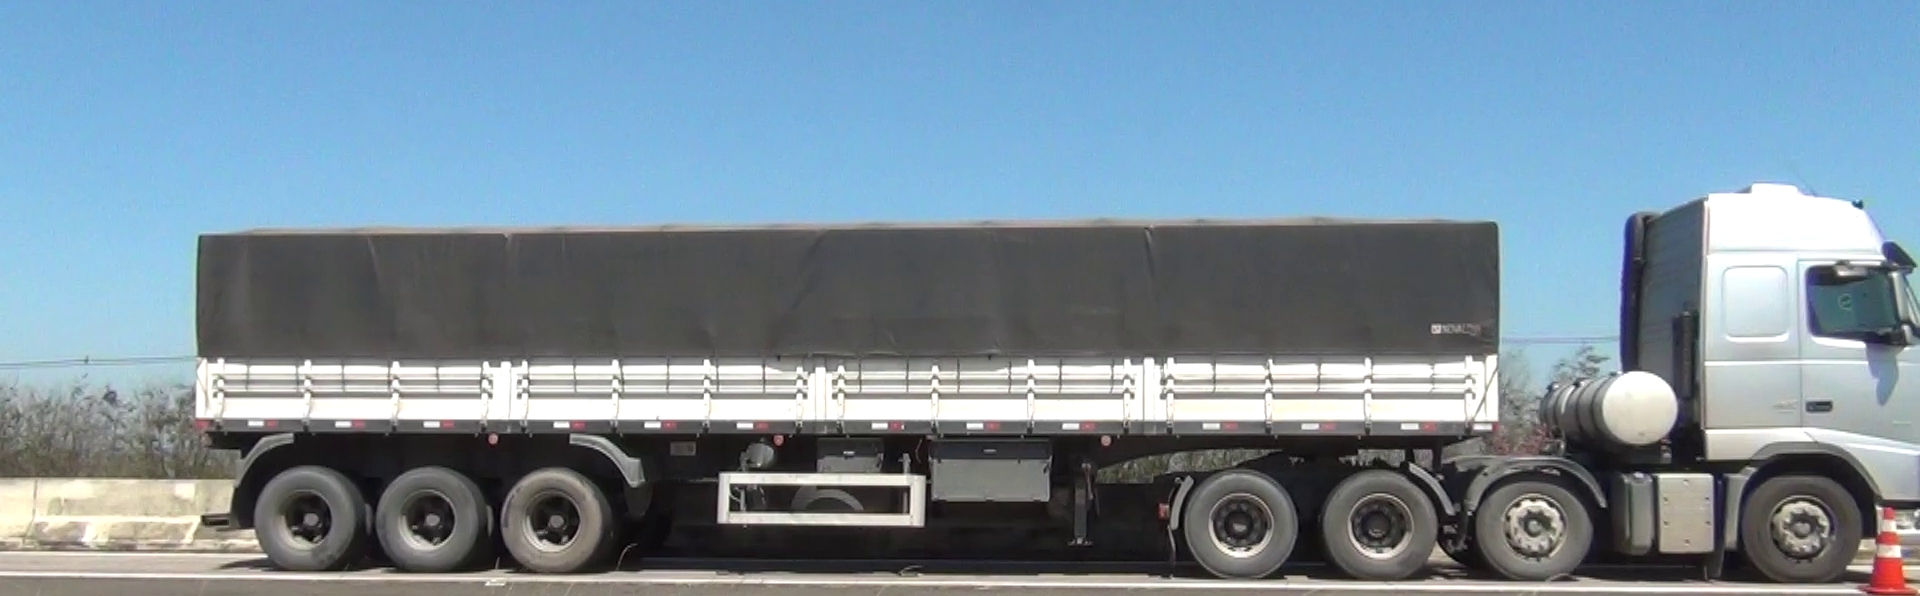
\includegraphics[width=.75\textwidth]{Images/20160927102749_color-[ROI-1]-1.jpg}
            \caption{Exemplo de imagem de caminhão}
            \label{fig:caminhaoExemplo}
        \end{figure}

    \subsection{Pré-processamento}

        Os autores do dataset não disponibilizaram uma separação padrão entre imagens de treino, validação e teste, somente a divisão de 9:1 de imagens de treino em relação a testes. Dessa forma, as imagens serão escolhidas aleatoriamente dentre o conjunto de dados.

        As imagens que foram selecionadas para o processo de treinamento passarão por uma etapa de \textit{data augmentation}, ocorrendo variações aleatórias nas características das imagens, como saturação, exposição, hue, inversão horizontal e adição de ruído aleatório.

        Com essas modificações, espera-se que o modelo fique mais robusto e consiga aprender melhor a identificar as características dos eixos, a fim de realizar melhores predições ao final.

    \subsection{Características do modelo implementado}
        Para este estudo, duas diferentes abordagens serão exploradas. A primeira, seguindo o desenvolvimento de \cite{Souza2024}, \cite{marcomini2023truckaxledetectionconvolutional} e \cite{Miles2022}, será utilizado a versão mais recente do YOLO, a YOLOv11 \cite{khanam2024yolov11overviewkeyarchitectural}, que apresenta uma melhoria de 2\% no tempo de predição em relação à YOLOv10 e possui 22\% menos parâmetros que a YOLOv8m, sendo mais eficiente e efetiva ao manter os níveis de acurácia. 
        
        Já a outra abordagem seguirá a ideia de uma rede convolucional padrão, como a utilizada em \cite{Almutairi2022}. Todavia, como a quantidade de de eixos varia de acordo com o tipo de caminhão, será utilizada uma regressão para computar a quantidade de eixos detectados na imagem, utilizando a loss MAE, que retorna o valor do erro na mesma unidade de medida.

    \subsection{Métricas de avaliação}
        Como métrica para avaliar os modelos treinados, serão utilizadas métricas de Precision (Indicando o quanto dos eixos identificados de fato eram eixos), Recall (Indicando quantas vezes o modelo não identificou um eixo onde de fato não deveria ter) e F1-Score, uma vez que, para base de dados desbalanceadas, o uso da acurácia pode não refletir corretamente a eficiência do modelo.
    

\section{References}
\bibliographystyle{sbc}

\bibliography{sbc-template}

\end{document}
